\documentclass[12pt]{article}

\usepackage[margin=1in]{geometry}
\usepackage{amsfonts,amsmath,amssymb}
\usepackage{multicol}

\usepackage{graphicx}
\usepackage{float}
\usepackage[nottoc, notlot, notlof]{tocbibind}
\usepackage{hyperref}
\usepackage{enumitem}
\usepackage{caption}
\usepackage{subcaption}
\usepackage[T1]{fontenc}
\usepackage[utf8]{inputenc}
\usepackage{xcolor}
\usepackage{pgfgantt}
\usepackage{rotating}
\usepackage[graphicx]{realboxes}

\newcommand{\leavealine}
{\vskip 0.5cm}


% for equation box
\usepackage{color}
\definecolor{myblue}{rgb}{.8, .8, 1}

\usepackage[most]{tcolorbox}
\tcbset{
	enhanced,
	colback=myblue!100!white,
	boxrule=0.1pt,
	colframe=myblue!100!black,
	fonttitle=\bfseries
}
%until here

% for python code
\usepackage[utf8]{inputenc}

% Default fixed font does not support bold face
\DeclareFixedFont{\ttb}{T1}{txtt}{bx}{n}{12} % for bold
\DeclareFixedFont{\ttm}{T1}{txtt}{m}{n}{12}  % for normal

% Custom colors
\definecolor{deepblue}{rgb}{0,0,0.5}
\definecolor{deepred}{rgb}{0.6,0,0}
\definecolor{deepgreen}{rgb}{0,0.5,0}

% \usepackage{listings}

% Python style for highlighting
\usepackage[utf8]{inputenc}

% Default fixed font does not support bold face
\DeclareFixedFont{\ttb}{T1}{txtt}{bx}{n}{12} % for bold
\DeclareFixedFont{\ttm}{T1}{txtt}{m}{n}{12}  % for normal

\DeclareSymbolFont{matha}{OML}{txmi}{m}{it}% txfonts
\DeclareMathSymbol{\varv}{\mathord}{matha}{118}
% Custom colors
\usepackage{color}
\definecolor{deepblue}{rgb}{0,0,0.5}
\definecolor{deepred}{rgb}{0.6,0,0}
\definecolor{deepgreen}{rgb}{0,0.5,0}
\definecolor{almostwhite}{rgb}{0.99,0.99, 0.99}

\usepackage{listings}

% Python style for highlighting
\lstset{
	basicstyle  =   \footnotesize,
	keywordstyle    = \color{deepred}\bfseries,
	stringstyle     = \color{strings},
	identifierstyle = \color{black},
	commentstyle    = \color{deepgreen},
	breaklines=true,
	numbersep=-10pt,
	stepnumber=1,
	showspaces=false,
	escapechar=§,
	showstringspaces=false,
	showtabs=false,
	frame=single,  
	rulecolor=\color{black},
	tabsize=4,              
	captionpos=t,           
	breaklines=true,
	breakatwhitespace=false,
	numbers=left,
	extendedchars=\true,
	emph=[3]{href, Particle, Boris_update, Field, uniform_E_field, radial_E_field, uniform_B_field, helmholtz_coil_B_field, two_helmholtz_B_field, Sampler, sample_uniform_position, sample_uniform_velocity, sample_velocity_uniformKE, sample_Maxwellian_velocity, sample_parabolic_velocity},
	emphstyle=[3]{\color{deepblue}},
	backgroundcolor=\color{almostwhite},
	language=Python 
}

%until here

%for gantt chart
\newganttchartelement*{mymilestone}{
	mymilestone/.style={
		shape=isosceles triangle,
		inner sep=0pt,
		draw=cyan,
		top color=white,
		bottom color=cyan!50
	},
	mymilestone incomplete/.style={
		/pgfgantt/mymilestone,
		draw=yellow,
		bottom color=yellow!50
	},
	mymilestone label font=\slshape,
	mymilestone left shift=0pt,
	mymilestone right shift=0pt
}

\newgantttimeslotformat{stardate}{%
	\def\decomposestardate##1.##2\relax{%
		\def\stardateyear{##1}\def\stardateday{##2}%
	}%
	\decomposestardate#1\relax%
	\pgfcalendardatetojulian{\stardateyear-01-01}{#2}%
	\advance#2 by-1\relax%
	\advance#2 by\stardateday\relax%
}


\begin{document}
	
	\fontfamily{ppl}\selectfont 
		\begin{center}
			\large{\textbf{MEE4099 Capstone Project}} \\ 
			\normalsize{Review 1 tentative report: first draft} \\
			\normalsize{Project Title:} \\ 
			\Large{\textbf{Magnetic Mirror Effect in Magnetron Plasma:}} \\
			\Large{\textbf{Modeling of Plasma Parameters}} \\
		\end{center}
		%\color{blue}
	\textbf{Project ID:} 21BTECH10051 \\
	\textbf{Team Members:} \\
	18BEM0145 Sashi Kant Shah \\
	18BME2104 Kaushal Timilsina \\
	18BME2109 Hrishav Mishra \\
	
	\noindent \textbf{Internal Guide:} \\
	Professor Sitaram Dash
	
	\tableofcontents
	\newpage
	
	\section{Introduction}
	One of the team members- 18BME2104 Kaushal studied the class MEE4005 Surface Engineering taught by Professor Sitaram Dash- our internal guide, during the Fall Semester 2021. Many interesting plasma based surface engineering techniques were studied during the class, one such technique being Magnetron Sputtering. This inspired the study of plasma in this project.
	
	\subsection{Plasma}
	One comes across many definitions of plasma including: fourth state of matter, ionized gas, a non equilibrium state of matter with dynamical characteristics due to electrodynamics, etc. However, it is best to describe plasma with some characteristic parameters, when one attempts to describe a plasma quantitatively. Some quantities that help define a plasma are:
	\begin{enumerate}
		\item Number density, $n$ \\
		Number density of a plasma describes the number of particles per unit volume. Plasma contains charged particles or ionized species. However, a plasma might at the same time also contain neutral atoms and molecules but also particles of different species- charged and neutral. If multiple species are contained in a plasma system, number densities of each species could be used to describe the system. For example, a plasma may contain electrons, charged ions and neutral atoms and molecules. Mass density $\varrho$ is defined as $\varrho := m n$ and is often used alongside number density, where $m$ is the mass of the species.
		
		\item Ionization, $\alpha$ \\
		Defined as $\alpha := \frac{\displaystyle n_{charged}}{\displaystyle n_{charged} + n_{neutral}}$, the ionization of a plasma describes the fraction of charged particles, with $\alpha = 1$ meaning that all the particles are charged and $\alpha = 0$ meaning that all the particles are neutral.
		
		\item Temperature, $T$ \\
		The temperature of a plasma describes the average kinetic energy of the particles in the plasma. When a gas is ionized to form a plasma, the ionization $\alpha$ can depend on the temperature of the plasma.
		
		\item Mean free path, $\lambda_{mfp}$ \\
		The gas-like behavior of a plasma is characterized by mean free path of particles much larger than the scale of the plasma. The mean free path is influenced by the temperature of the plasma. The mean free path and the thermal velocity of the particles as described by the temperature, are related by the timescale of collisions as $\lambda := v_{th} \tau$ where $\tau$ is the timescale of collisions. 
		
		\item Debye Length, $\lambda_{D}$ \\
		In a plasma, electrostatic Coulomb interactions between charged particles compete with random thermal speed of the particles described by the temperature of the plasma. The Debye sphere is an imaginary sphere around a charged particle, where oppositely charged particles are attracted and in doing so screen the charge of the central particle to the outer plasma so that the electrostatic influence of a particle is limited to the Debye sphere surrounding it. This is why plasma's are often said to be Quasi-neutral as charge screening leads to a neutral behavior electrostatically on a scale much larger than the Debye length. The Debye length is defined as the radius of the Debye sphere.
		
		\item Plasma beta parameter, $\beta$ \\
		The beta parameter defined as $\beta := \frac{\displaystyle 8 \pi n T}{\displaystyle B^{2}}$ describes the ratio of the thermal and magnetic energies of the plasma, as particles in random thermal motions compete with the Lorentz force.
		
	\end{enumerate} 
		Many other parameters like the Larmor radius, quantities like frequencies of different waves describing the dynamics; are also important in describing a plasma. However, as we shall see later; particles in the plasma are more important to this project than many interesting parameters describing the plasma.
	
	\subsection{Laboratory Plasma}
	Laboratory plasmas are often characterized by some properties like:
	\begin{itemize}[itemsep=0cm]
		\item High ionization fraction
		\item Sub atmospheric pressure required to sustain ionization
		\item Temperature range : 1000 - 30000 K
	\end{itemize}

	\noindent Many surface engineering processes use plasmas to obtain high performance coatings. Some processes that use plasma are:
	\begin{enumerate}[itemsep=0cm]
		\item Plasma Immersion Ion Implantation
		\item Plasma Enhanced Chemical Vapor Deposition
		\item Magnetron Sputtering (PVD)
		\item Air Plasma Spray (Spray technique)
		\item Plasma Transferred Arc (Hardfacing technique)
	\end{enumerate}
	
	\subsection{Physical Vapor Deposition}
	Physical Vapor Deposition(PVD) is a family of surface engineering techniques where thin film coatings are grown on the surface of a specimen, in a vacuum chamber. Particles from a vapor move around on the surface of the specimen as random walkers and eventually get trapped in strained pockets producing nucleation site for the growth of a film. Most PVD techniques fall under either of the two catgories:
	\begin{enumerate}
		\item Evaporation techniques \\
		Evaporation techniques involve heating the material to  to a high temperature when it forms vapor and the particles in the vapor are coated on the substrate. It is for that reason that evaporation techniques are called hot techniques. Semiconductors like Si/Ge, insulators like oxides and metals like Tungsten are often coated on substrates using evaporation techniques. 
		
		\item Sputtering techniques \\
		Sputtering techniques on the other hand are known as cold techniques. Sputtering techniques use a high energy beam to remove material from a target and the removed material is coated on the required substrate.
		
	\end{enumerate}

	\subsection{Magnetron Sputtering}
	Magnetron sputtering is a sputtering technique where the sputtered ions form a magnetically confined plasma. The plasma, controlled by magnetic fields, transports the ions to the surface of the substrate forming the coating. 
	
	
	\begin{figure}[H]
		\begin{center}
			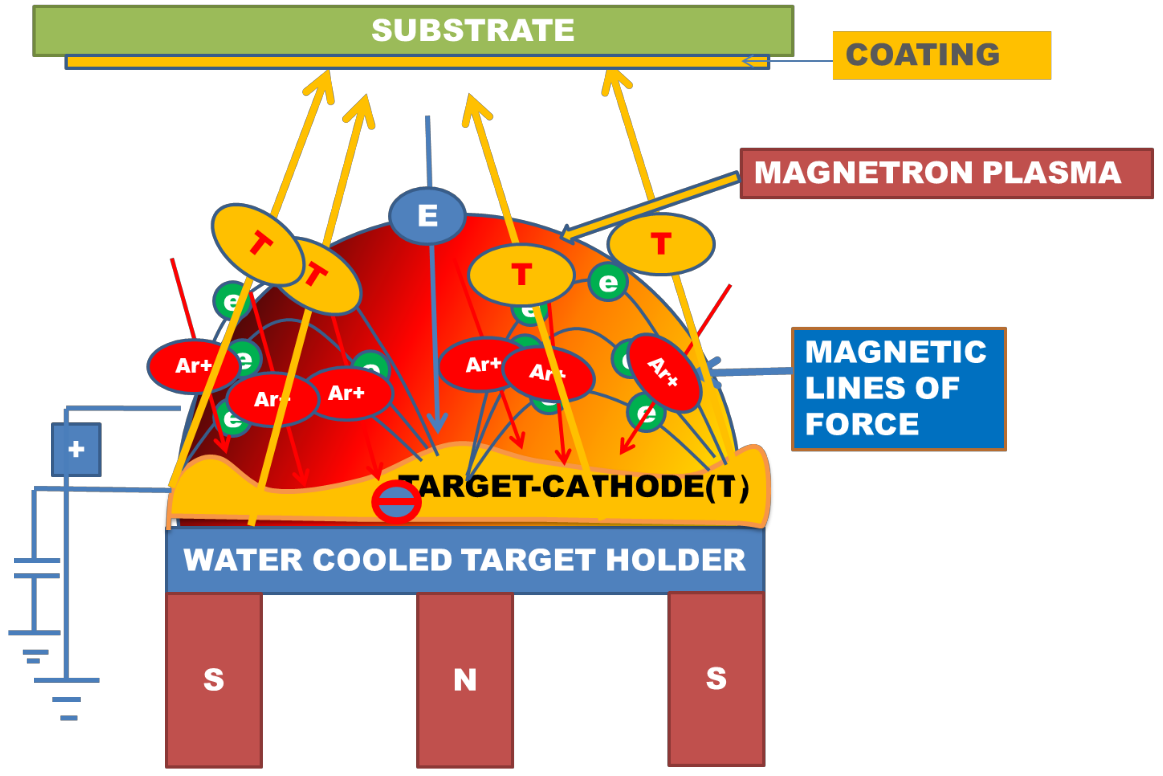
\includegraphics[width=12cm, height=8cm]{magnetron sputtering.png} \caption{Magnetron Sputtering system. credit: \cite{SurfaceEng}}
		\end{center}
	\end{figure}
	
	\subsection{Magnetic Mirror}
	The magnetic mirror effect can first be illustrated with a 	single particle. For the simple case, it is assumed that there is no electric field acting on the particle, the magnetic field is cylindrically symmetric and the gradient of the magnetic field is only along the axial direction of the cylinder, the $z$ direction.  The magnetic moment $$\mu = \frac{m v_{\perp}^{2}}{2B_{z}} $$ of the particle is an adiabatic invariant of the particle motion and hence is approximately conserved for a magnetic field whose $z$ component $B_{z}$ does not vary too much . The kinetic energy$$ KE = \frac{1}{2}m v^{2}$$ of the particle is also approximately conserved. Writing $v_{\perp} = v sin \theta$,
	$$\frac{\mu}{KE} = \frac{sin^{2}\theta}{B_{z}}$$ is also a conserved quantity. This means that as $B$ increases (within a small range), $sin^{2}\theta$ increases as well and so does $|sin\theta|$ which means that $|v_{\perp}|$ increases and since $v$ is conserved, $v_{\parallel}$ decreases to zero. When $v_{\parallel} = 0$, the particle is no longer moving in the $z$ direction, but is moving with velocity $v$ in the plane perpendicular to $z$ direction. The $v_{\parallel}$ then increases in the opposite direction as the particle moves towards decreasing $B$ because of the Lorentz force. Such a particle is seen as being reflected due to the configuration of the magnetic field and hence such a configuration of the magnetic field is called a magnetic mirror. Particles whose $v_{\parallel}$ does not decrease to 0 while the value of $B$ is decreasing, escape from the magnetic mirror configuration. \\
	
	\noindent A magnetic mirror configuration is important in a magnetic plasma trap chamber such as that used in Magnetron sputtering. Particles in a plasma have different speeds depending on the initial distribution which is based on parameters like the plasma temperature. The speeds of particles change depending on the electric and magnetic fields. Based on the magnetic mirror effect, one can determine which particle (having certain velocities) can escape the magnetic trap and which of those are reflected. The less the particles escape the magnetic trap, the more of the flux is used in forming coatings and less of the ionized gas is wasted. This is very useful in understanding the required gas supply and rate of deposition.
	
	\section{Literature Review}
	A large part of the literature review for the project consisted of studying basic plasma physics in order to understand how we could formulate the project and proceed ahead. 
	
	\subsection{Plasma as a system}
	Various models are used to describe Plasma as a system. Some of the common approaches are:
	\begin{enumerate}
		\item \textbf{Single particle description} \\
		This model is used to describe the motion of a charged particle under the influence of electric and magnetic fields. The particle's motion is described by the Lorentz force 
		\begin{equation}
			\label{eqn:lorentz}
			\frac{d \textbf{$\boldsymbol{v}$}}{d t} = \frac{q}{m} \left(\textbf{$\mathbf{E}$} + \textbf{$\boldsymbol{v}$} \times \textbf{$\mathbf{B}$} \right)
		\end{equation}
		Describing many particles evolving under the influence of Lorentz force, it is easy to describe a plasma assuming that the mean free path of the particles is much larger than the dimensions of the chamber; meaning that particles hardly ever collide. This is to say that in the simplest case, under this model particles evolve under the influence of electric and magnetic fields but the particles do not produce any electric and magnetic fields of their own or affect the external applied fields and hence also do not interact with other particles.
	
		\item \textbf{Kinetic theory} \\
		The kinetic theory describes the plasma as collection of particles whose state (position and velocity) is treated as a random variable with a density function \\ $ f(x, y, z, v_{x}, v_{y}, v_{z}, t) $ which describes the number of particles at position $ (x, y, z) $ at time $ t $ with velocities between $ v_{x} $ and $ v_{x} + dv_{x} $, $ v_{y} $ and $ v_{y} + dv_{y} $, $ v_{z} $ and $ v_{z} + dv_{z} $ in directions $x$, $y$ and $z$ respectively. For a simpler notation $ f(x, y, z, v_{x}, v_{y}, v_{z}, t) $ is denoted as $ f(\boldsymbol{x}, \boldsymbol{v}, t) $.
		The expression $$\displaystyle \int_{all \hspace{0.2cm} v_{x}^{}} dv_{x} \int_{all \hspace{0.2cm} v_{y}^{}} dv_{y} \int_{all \hspace{0.2cm} v_{z}^{}} dv_{z} f(\boldsymbol{x}, \boldsymbol{v}, t) $$ gives the number of particles at position $\boldsymbol{x}$, at time $t$.  For a simple choice of notation, it if often written as $$\displaystyle \int_{all \hspace{0.2cm} \boldsymbol{v}^{}} d^{3}v f(\boldsymbol{x}, \boldsymbol{v}, t) \hspace{0.5cm}\mathnormal{or} \hspace{0.5cm}\int_{all \hspace{0.2cm} \boldsymbol{v}^{}} d\boldsymbol{v} f(\boldsymbol{x}, \boldsymbol{v}, t)$$ A density function is said to be normalized if $$\displaystyle \int_{all \hspace{0.2cm} \boldsymbol{v}^{}} d\boldsymbol{v} f(\boldsymbol{x}, \boldsymbol{v}, t) = 1$$ Such a density function is also denoted with a hat as $ \hat{f}(\boldsymbol{x}, \boldsymbol{v}, t) $.\\
		\noindent The average velocity $\bar{v}$ for a density function $ \hat{f}(\boldsymbol{x}, \boldsymbol{v}, t) $ is calculated as  $$\displaystyle \int_{all \hspace{0.2cm} \boldsymbol{v}^{}} d\boldsymbol{v} \hspace{0.2cm} v f(\boldsymbol{x}, \boldsymbol{v}, t)$$ Various other features of the distribution are: the Root Mean Square velocity $v_{rms}$, the average absolute velocity $|\bar{v}|$, the average velocity in $z$ direction $\bar{v_{z}}$, etc.\\
		The evolution of the particles is described as the changing of the density function. Boltzmann equation is often used to describe this dynamics:
		
		$$\frac{\partial f}{\partial t} + \boldsymbol{v} \cdot \nabla f + \frac{\mathbf{F}}{m} \cdot {\partial}_{\boldsymbol{v}} f = \left(\frac{\partial f}{\partial t}\right)_{c}$$
		While it may look complicated at first, the left hand side of the equation is actually just a short form for
		$$ \frac{df}{dt} = \frac{\partial f}{\partial t} + \frac{\partial f}{\partial x} v_{x} + \frac{\partial f}{\partial v_{x}} a_{x} + \frac{\partial f}{\partial y} v_{y} + \frac{\partial f}{\partial v_{y}} a_{y} + \frac{\partial f}{\partial z} v_{z} + \frac{\partial f}{\partial v_{z}} a_{z}$$
		which is just
		$$ \frac{df}{dt} = \frac{\partial f}{\partial t} + \frac{\partial f}{\partial x} \frac{d x}{d t} + \frac{\partial f}{\partial v_{x}} \frac{d v_{x}}{d t} + \frac{\partial f}{\partial y} \frac{d y}{d t} + \frac{\partial f}{\partial v_{y}} \frac{d v_{y}}{d t} + \frac{\partial f}{\partial z} \frac{d z}{d t} + \frac{\partial f}{\partial v_{z}} \frac{d v_{z}}{d t}$$
		For simplicity, let us look at the 1-dimensional (2-phase dimensional) version of this expression:
		$$ \frac{df}{dt} = \frac{\partial f}{\partial t} + \frac{\partial f}{\partial x} \frac{d x}{d t} + \frac{\partial f}{\partial v_{x}} \frac{d v_{x}}{d t}$$
		If the right hand side of the Boltzmann equation were zero, in 1-dimension (2-phase dimensions), it would read:
		$$\frac{df}{dt} = 0$$
		This would mean that the distribution function is unchanging (in its own frame). If particles were not interacting and there was no external disturbance, this is exactly what would happen. This is why with the expression on the right hand side set to zero, the Boltzmann equation is said to be collisionless. Adding a non zero expression on the right hand side would account for interactions between the particles or the effect of external disturbances. 
		
		\item \textbf{Fluid model} \\
		The fluid model is describes the plasma in terms of macroscopic variables like Pressure, Temperature, average velocity, density, flux; like ordinary fluid dynamics. The governing Partial Differential Equations are obtained by taking moments of the Boltzmann equation, or a special case of the Boltzmann equation called the Vlasov equation. Such a procedure gives rise to: \\
		
		The continuity equation: \\
		$$\frac{\partial \varrho}{\partial t} + \boldsymbol{\nabla} \cdot \left(\varrho \boldsymbol{v}\right) = 0$$
		and the Cauchy momentum equation: \\
		$$\varrho \left(\frac{\partial}{\partial t} + \boldsymbol{v} \cdot \boldsymbol{\nabla}  \right) \boldsymbol{v} = \mathbf{J} \times \mathbf{B} - \boldsymbol{\nabla} p$$
		Higher moments yield other equations for quantities like the entropy. The fluid equations average over the velocity distribution of the particles to obtain the macroscopic variables like Pressure and Temperature, as discussed earlier- by taking moments of the Kinetic equations like the Boltzmann equation or the Vlasov equation.
		
		\item \textbf{Magnetohydrodynamics} \\
		Magnetohydrodynamics(MHD) is an extension of the fluid model of describing a plasma. In a first approximation, the magnetic and electric fields acting on the fluid and the currents generated are now solved using Faraday's law: \\
		$$\frac{\partial \mathbf{B}}{\partial t} = - \boldsymbol{\nabla} \times \mathbf{E}$$
		and the Ampere's law: \\
		$$\mu_{0} \mathbf{J} = \boldsymbol{\nabla} \times \mathbf{B}$$
		The full set of Maxwell's equations can also be coupled with the fluid. MHD description of a plasma also describes dynamic waves such as Alfv\'en waves and magnetosonic waves. MHD theory can also be used to describe interaction of the plasma with electromagnetic waves, for example those from a LASER source relevant to LASER plasma processes in surface engineering. Ideal MHD studies plasma as a fluid of single species, however, multi-species plasma can also be studied. \\
		
		\item \textbf{The model used in the project} \\
		In the context of plasma processes like Magnetron Sputtering where particles have a considerably large mean free path, we have decided not to use the fluid model and the MHD descriptions of a plasma. In such processes, it is almost always the case that the strength of the electric and magnetic fields applied by the apparatus is far more stronger than the electric and magnetic fields generated by charged particles in a plasma. This approximation allows us to avoid solving Maxwell's equations and use only the Lorentz force. The model used in the project is mostly similar to the single particle model, where in a collection of particles, each particle evolves under the influence of the electric and magnetic fields set up by the apparatus; governed by the Lorentz force. However, we incorporate a little bit of the Kinetic theory in that we are interested in different initial velocity distributions for particles in the plasma and how the velocity distribution changes over time; as it is important to understand the velocity distribution to characterize the reflection and loss of particles in a magnetic-mirror like trap that may be setup in the plasma chamber.  
		
	\end{enumerate}
	
	\section{Gaps in Literature}
	It would take a number of courses on plasma physics to fully understand the current research methods in plasma physics. In the interest of time, we have studied some simple setups; so that we can setup well functioning plasma configuration during the course of the project and study some aspects that we are interested in. The forefront of research in plasma physics concerns complicated devices like Magnetic Confinement Fusion, or Quantum Optic systems. Most research in surface engineering focuses on the properties of coatings obtained and parameters of plasma used; in processes that use plasma. In our project, we would like to set up a simple plasma simulation that can help us study smaller devices like the one available in the School of Mechanical Engineering; where we can control a small flux of particles by tuning the electric and magnetic fields. This section describes, how we construct a simple easy to use, plasma simulation system; which is yet to be functional.
	
	\subsection{Particle in Cell Methods}
	Particle in a cell methods are used to simulate the kinetic theory of plasma. A simple strategy used for particle in cell plasma simulation based on strategies as outlined in the paper \cite{PIC good} and the slides \cite{PIC IAS} involves the following steps:
	\begin{enumerate}
		\item \textbf{Sampling and Initialization} \\
		The initial positions and velocities of particles in the plasma are sampled from a distribution, or based on some strategy.
		\item \textbf{Action of fields on the particles} \\
		The particles move under the influence of electric and magnetic fields as described by the Lorentz force as stated in the equation \eqref{eqn:lorentz}.
		\item \textbf{Particle deposition} \\
		In this step, charged particles are deposited on the grid defined by the mesh, and the charge density $\varrho_{i}$ and the current density $\boldsymbol{j}_{i}$ generated by the deposited particles is computed. One strategy outlined in the paper \cite{PIC good} defines charge deposition as following.
		$\boldsymbol{x_{i}} = \left(\boldsymbol{i} + 1/2\right) \Delta \boldsymbol{x}$, $\boldsymbol{i} \in \mathbb{Z}^{D}$ define the grid. A second order deposition can be achieved by:
		$$\varrho_{i} = \sum_{p}^{}\left(\frac{q_{p}}{V_{i}}\right) \mathbf{W_{2}} \left(\frac{\boldsymbol{x_{i}} - \boldsymbol{x_{p}}}{\Delta x}\right)$$
		where $V_{i} = \Delta x^{D}$ is the volume of the cell $i$ and $\mathbf{W_{2}}\left(\boldsymbol{x}\right)$ is a $D$-dimensional interpolating function defined in \cite{PIC good}. In simple models, the current density $\boldsymbol{j}_{i}$ is often not used.
		\item \textbf{Fields generated by particles} \\
		In this step, the electric and magnetic fields generated by the charge density and current density are computed. The paper \cite{PIC good} uses Poisson equation to compute the electric field generated by the charge distribution and neglects the magnetic field generated. However, in high performance simulations like that outlined in \cite{PIC IAS}, the full set of Maxwell's equations are used to compute the electric and magnetic fields generated by the particles.
		\item \textbf{Force on particles} \\
		In this step, the force on the particles due to the electric and magnetic fields are computed. Most simulations like the one outlined in the paper \cite{PIC good}; because they compute the electric and magnetic fields generated by the deposited particles, are able to describe the interaction of each particle with the electric and magnetic fields generated by other particles in the plasma, and hence capture the particle-particle dynamics.
		\item \textbf{Action of the force on particles} \\
		Step 2 is repeated to move the particles under the influence of the electric and magnetic fields.
	\end{enumerate}

	A flow-chart for the simulation based on a similar strategy outlined in \cite{PIC IAS} is presented below.

	\begin{figure}[H]
		\begin{center}
			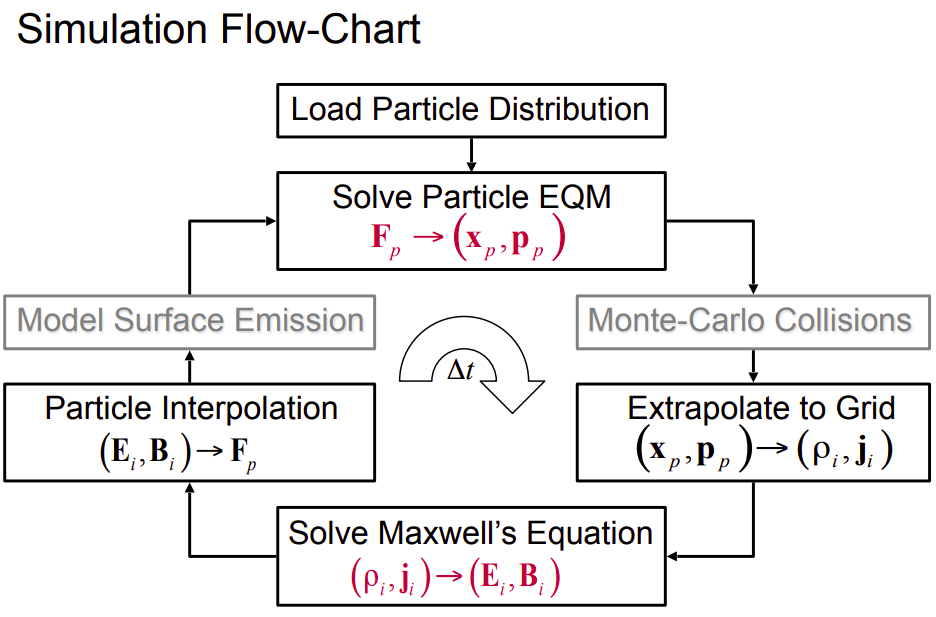
\includegraphics[width=12cm, height=8cm]{PIC.png} \caption{Flowchart for PIC methods. credit: \cite{PIC IAS}}
		\end{center}
	\end{figure}
	
	\section{Problem Definition}
	Our approach is similar to and differs from the general procedure outlined for Particle in Cell methods, in the following ways:
	\begin{enumerate}
		\item \textbf{Sampling and Initialization} \hspace*{\fill}Similar \phantom{text} \\
		This step is similar to the first step in general PIC methods. We sample the initial positions and velocities of the particles based on some strategies like sampling from the Maxwell-Boltzmann distribution or uniform initialization strategies described in Methodology.
		\item \textbf{Action of fields on the particles} \hspace*{\fill}Similar \phantom{text}\\
		This step is similar to the second step in general PIC methods. We update the positions and particles of the particles according to the Boris Algorithm, based on the Lorentz force; as described in Methodology.
		\item \textbf{Particle deposition} \hspace*{\fill}Skipped \phantom{text}\\
		We skip this step in our approach for reasons described in the next step.
		\item \textbf{Fields generated} \hspace*{\fill}Different \phantom{text} \\
		As discussed earlier; when discussing the model used in the project, in devices such as those used in surface engineering processes, it is often the case that the electric and magnetic fields generated by the apparatus are far more stronger than those generated by the particles. So it is reasonable to assume that the fields generated by the particles are negligible compared to the fields generated by the apparatus. While general PIC methods compute fields generated by particles in the plasma, we only used fields generated by the apparatus. Since we neglect the fields generated by the particles in the plasma, we can skip depositing particles in the grid; which would be the third step of general outline of PIC methods. This makes our model simpler and easier to work with, evaluate and understand. We define the fields generated by the apparatus or field configurations based on analytic configurations and move the particles in the plasma under their influence. This is later described in methodology. 
		\item \textbf{Force on particles} \hspace*{\fill}Skipped \phantom{text} \\
		As we do not compute the electric and magnetic fields generated by the particles, this step is skipped and the action of the electric and magnetic fields created by the apparatus is done directly in step 6. 
		\item \textbf{Action of the fields on particles} \hspace*{\fill}Similar \phantom{text} \\
		Similar to the sixth step of general PIC methods, we repeat step 2 to move the particles under the influence of electric and magnetic fields created by the apparatus.
	\end{enumerate}

	\noindent Our approach can be summarized in the following set of steps: \\
	\phantom{te} Do for each batch of particles in the plasma stream:
	\begin{enumerate}[itemsep=0cm]
		\item \textbf{Sampling and Initialization} \hspace*{\fill}Kinetic Theory \phantom{text}
		\item \textbf{Definition of fields} \hspace*{\fill}Apparatus \phantom{text} \\
		If required use a different field to simulate control of the apparatus, for example: changing the voltage of the electrode; changing the electric field.
		\vspace{0.2cm} \\Do for certain number of time steps:
		
		\begin{itemize}[itemsep=0cm]
			\item \textbf{Particle update based on Lorentz force} \hspace*{\fill}Single particle dynamics \phantom{text}
		\end{itemize}
		\item \textbf{Remove particles} \hspace*{\fill}Surface Engineering process \phantom{text}\\
		Particles are either absorbed to form a coating or exit the plasma chamber.
	\end{enumerate}
	The details are described later in methodology. The steps of our approach as described help us define our objectives as discussed in the following section.
	
	\section{Objectives}
	The objectives of the project are based on our approach to the problem as described in problem definition:
	\begin{enumerate}
		\item \textbf{Single Particle Method} \\ 
		To simulate charged particles that evolve under the influence of electric and magnetic fields; as governed by the Lorentz force.
		\item \textbf{Field Configurations} \\
		To simulate a few different configurations of electric and magnetic fields- some describing apparatus like coils; some describing analytic expressions for fields and to study the different evolution of particles.
		\item \textbf{Kinetic Theory} \\
		To study different initial velocity distributions and how the velocity distribution of particles changes as the particles evolve. Parameters like the Plasma temperature are to be studied under this topic.
		\item \textbf{Analysis} \\
		To analyze different batches or collections of particles, subjected to different field configurations.
		
	\end{enumerate}
	
	\section{Methodology}
	
	\subsection{Particle Evolution- single particle dynamics}
	As discussed earlier, we evolve individual particles in the plasma with the Lorentz force. To achieve this in a simulation, the Lorentz force equations are discretized and then solved using the Boris Algorithm; a standard algorithm for simulating charged particles in electric and magnetic fields.

	\subsubsection{Lorentz Force}
	The equations of motion for a charged particle under the influence of Electric and Magnetic fields is described by the Lorentz Force in the S.I. units as
	$$
		\frac{d \textbf{$\boldsymbol{v}$}}{d t} = \frac{q}{m} \left(\textbf{$\mathbf{E}$} + \textbf{$\boldsymbol{v}$} \times \textbf{$\mathbf{B}$} \right)
	$$ as discussed earlier in equation $\left(\ref{eqn:lorentz}\right)$;
	along with the expression for the velocity
	\begin{equation}
		\label{eqn:velocity}
		\frac{d \boldsymbol{x}}{d t} = \boldsymbol{v}
	\end{equation} 
	
	\noindent These equations are discretized to obtain
	\begin{equation}
		\label{eqn:Dlorentz}
		\frac{\boldsymbol{v}_{k+1} - \boldsymbol{v}_{k}}{\Delta t} = \frac{q}{m} \left[\mathbf{E}_{k} + \frac{\left( \boldsymbol{v}_{k+1} + \boldsymbol{v}_{k} \right) }{2} \times \mathbf{B}_{k} \right] 
	\end{equation}
	from the Lorentz Force equation ( \ref{eqn:lorentz} ), and
	\begin{equation}
		\label{eqn:Dvelocity}
		\frac{\boldsymbol{x}_{k+1} - \boldsymbol{x}_{k} }{\Delta t} =	\boldsymbol{v}_{k+1}
	\end{equation}
	from the expression for velocity in equation ( \ref{eqn:velocity} ), where the subscript $k$ denotes the $k$-th time step.
	
	
	\subsubsection{Boris Algorithm}
	The discretized Lorentz equations may be solved using the Boris Algorithm, as we do in this project.
	The Boris Algorithm splits equation (\ref{eqn:Dlorentz}) into three equations.
	\begin{equation}
		\label{eqn:halfEpulse1}
		\frac{\boldsymbol{v}^{-} - \boldsymbol{v}_{k}}{\left( \Delta t  / 2 \right)} = \frac{q}{m} \mathbf{E}_{k} \hspace{1cm} or \hspace{1cm}	
		\frac{\boldsymbol{v}^{-} - \boldsymbol{v}_{k}}{ \Delta t } = \frac{1}{2}\frac{q}{m} \mathbf{E}_{k}
	\end{equation}
	which is often called the first half of the electric pulse.
	\begin{equation}
		\label{eqn:Brotation}
		\frac{\boldsymbol{v}^{+} - \boldsymbol{v}^{-}}{ \Delta t } = \frac{q}{m} \left(\frac{\boldsymbol{v}^{+} + \boldsymbol{v}^{-}}{ 2 }\right) \mathbf{B}_{k}
	\end{equation}
	which is often called rotation by the magnetic field.
	\begin{equation}
		\label{eqn:halfEpulse2}
		\frac{\boldsymbol{v}_{k+1} - \boldsymbol{v}^{+}}{\left( \Delta t  / 2 \right)} = \frac{q}{m} \mathbf{E}_{k} \hspace{1cm} or \hspace{1cm}	
		\frac{\boldsymbol{v}_{k+1} - \boldsymbol{v}^{+}}{ \Delta t } = \frac{1}{2}\frac{q}{m} \mathbf{E}_{k}
	\end{equation}
	which is often called the second half of the electric pulse.
	
	\noindent Adding equations (\ref{eqn:halfEpulse1}), (\ref{eqn:Brotation}) and (\ref{eqn:halfEpulse2}) gives
	$$ \label{eqn:Dlorentz}
	\frac{\boldsymbol{v}_{k+1} - \boldsymbol{v}_{k}}{\Delta t} = \frac{q}{m} \left[\mathbf{E}_{k} + \frac{\left( \boldsymbol{v}^{+} + \boldsymbol{v}^{-} \right) }{2} \times \mathbf{B}_{k} \right] $$ which is almost the discretized Lorentz equation ( \ref{eqn:Dlorentz}) except that $\left( \boldsymbol{v}^{+} + \boldsymbol{v}^{-} \right) $ is substituted for $\left( \boldsymbol{v}_{k+1} + \boldsymbol{v}_{k}\right) $. However, subtracting equation (\ref{eqn:halfEpulse1}) from equation (\ref{eqn:halfEpulse2}) gives $\left( \boldsymbol{v}^{+} + \boldsymbol{v}^{-} \right) = \left( \boldsymbol{v}_{k+1} + \boldsymbol{v}_{k}\right) $, giving the discretized Lorentz equation ( \ref{eqn:Dlorentz} ). This means that the Boris algorithm is equivalent to the discretized Lorentz equation. \\
	
	\noindent
	The equations (\ref{eqn:halfEpulse1}), (\ref{eqn:Brotation}) and (\ref{eqn:halfEpulse2}) can be written slightly different as 
	
	\begin{center}
		\begin{tcolorbox}[width=8cm]
			
			\begin{equation}
				\begin{split}
					\boldsymbol{v}^{-} & = \boldsymbol{v}_{k} + q^{\prime} \mathbf{E}_{k} \\
					\boldsymbol{v}^{+} & = \boldsymbol{v}^{-} + 2 q^{\prime} \left( \boldsymbol{v}^{-} \times \mathbf{B}_{k} \right) \\
					\boldsymbol{v}_{k+1} & = \boldsymbol{v}^{+} + q^{\prime} \mathbf{E}_{k} \\
					\boldsymbol{x}_{k+1} & = \boldsymbol{x}_{k} + \Delta t \hspace{0.2cm}\boldsymbol{v}_{k+1}
				\end{split}	 			
			\end{equation}
		\end{tcolorbox}
	\end{center}
	
	alongwith equation (\ref{eqn:Dvelocity}) where $q^{\prime} = \frac{\displaystyle q}{\displaystyle m} \frac{\displaystyle \Delta t}{ 2}$. These equations are used to update the velocity of the particle under the influence of the Lorentz force under the Boris update strategy.
	
	\subsection{Particle Sampling- kinetic theory}
	As discussed earlier, kinetic theory of plasma uses density function and its evolution to describe a plasma. We pointed out that we will be using some aspects of kinetic theory in our project; in that we will initialize the batches (collections) of particles based on certain distributions. This will allow us to study parameters like the plasma temperature, in our project. \\
	
	\subsubsection{Maxwellian distribution}
	\noindent One important density function often used in the kinetic theory of plasma is the Maxwell-Boltzmann distribution often called the Maxwellian which has the density function 
	\begin{equation}
		\label{eqn:maxwellian}
		\widehat{f_{M}} := \hat{f}(\boldsymbol{x}, \boldsymbol{v}, t) = \left(\frac{m}{2\pi KT}\right)^{\frac{3}{2}} \mathrm{exp}\left(-\frac{v^{2}}{v_{th}^{2}}\right)
	\end{equation} where $$v_{th}^{2} = \frac{2 K T}{m}$$ Some features of the Maxwellian are:
	$$ v_{rms} = \sqrt{\frac{3 K T}{m}} \mathrm{,} |\bar{v}| = 2\sqrt{\frac{2 K T}{\pi m}} \mathrm{,} |\bar{v_{z}}| = \sqrt{\frac{2 K T}{\pi m}} \mathrm{,} \bar{v_{z}} = 0 $$
	
	\subsubsection{Parabolic distributions}
	We are also interested in defining other density functions to do the sampling. The simplest density function to try would be to have all particles have the same velocity i.e. a Dirac delta function distribution. Another simple distribution would be a uniform distribution between two velocities, where a particle is equally likely to have any velocity in the range.
	
	\begin{figure}[H]
		\begin{multicols}{2}
			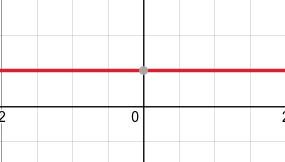
\includegraphics[width=\linewidth, height=5cm]{uniform.png} \caption{$f_{0}$} \par
			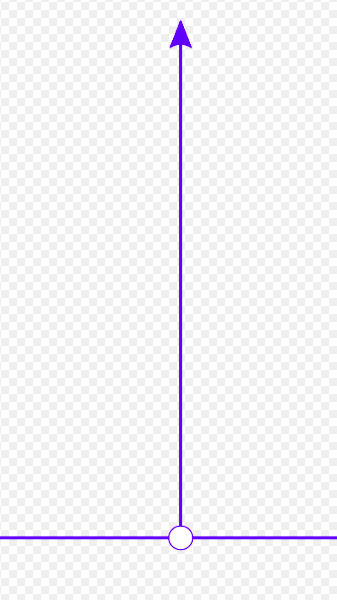
\includegraphics[width=\linewidth, height=5cm]{dirac.png} \caption{$f_{\delta}$} \par
		\end{multicols}
	\end{figure}
	Functions that look like $f_{0}$ might define he uniform distribution while functions like $f_{\delta}$ might describe the Dirac delta distribution. The figure for $f_{0}$ was generated using desmos graphing calculator while the figure for $f_{\delta}$ was snipped from the image in wikipedia for the Dirac delta function. We define initialization strategies based on uniform and Dirac delta distributions in our simulations.  \\
	
	\noindent Parabolic functions in a given range also seem like interesting distributions and yet simple to work with. After some trial and error, two functions that seem interesting are:
	\[ f_{1} = 
	\begin{cases} 
		1- \frac{v^{2}}{2 v_{a}^2} & -v_{a}\leq v\leq v_{a} \\
		0 & else 
	\end{cases}
	\]
	\[ f_{2} = 
	\begin{cases}
		1 + \frac{v^{2}}{2 v_{a}^2} & v_{a}\leq v\leq v_{a} \\
		0 & else
	\end{cases}\]  
	
	These functions can be normalized as
	$$ \int_{v_{x} = -v_{a}}^{v_{x} = v_{a}} dv_{x} \int_{v_{y} = -v_{a}}^{v_{y} = v_{a}} dv_{y} \int_{v_{z} = -v_{a}}^{v_{z} = v_{a}} dv_{z} \hspace{0.2cm}c_{0}  \left(1 - \frac{v_{x}^{2}+v_{y}^{2}+v_{z}^{2}}{2 v_{a}^2}\right) = 1 \hspace{2cm} \mathrm{and}$$
	$$ \int_{v_{x} = -v_{a}}^{v_{x} = v_{a}} dv_{x} \int_{v_{y} = -v_{a}}^{v_{y} = v_{a}} dv_{y} \int_{v_{z} = -v_{a}}^{v_{z} = v_{a}} dv_{z} \hspace{0.2cm} c_{0}  \left(1 + \frac{v_{x}^{2}+v_{y}^{2}+v_{z}^{2}}{2 v_{a}^2}\right) = 1 \hspace{2cm} \mathrm{giving}$$
	
	\[ \hat{f_{1}} = 
	\begin{cases} 
		\frac{1}{4 v_{a}^{3}} \left(1 - \frac{v^{2}}{2 v_{a}^2}\right) & -v_{a}\leq v\leq v_{a} \\
		0 & else 
	\end{cases}
	\]
	\[ \hat{f_{2}} = 
	\begin{cases}
		\frac{1}{12 v_{a}^{3}} \left(1 + \frac{v^{2}}{2 v_{a}^2}\right) & v_{a}\leq v\leq v_{a} \\
		0 & else
	\end{cases}\] 
	
	\noindent The graph of these functions (considering $v$ as a single variable) were generated using desmos graphing calculator. The figures represent $\hat{f_{1}}$ and $\hat{f_{2}}$ extrapolated to beyond the defined range.
	\begin{figure}[H]
		\begin{multicols}{2}
			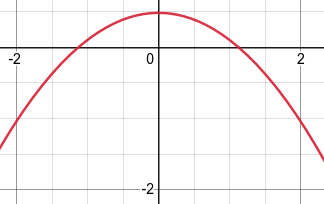
\includegraphics[width=\linewidth, height=5cm]{first.png} \caption{$\hat{f_{1}}$} \par
			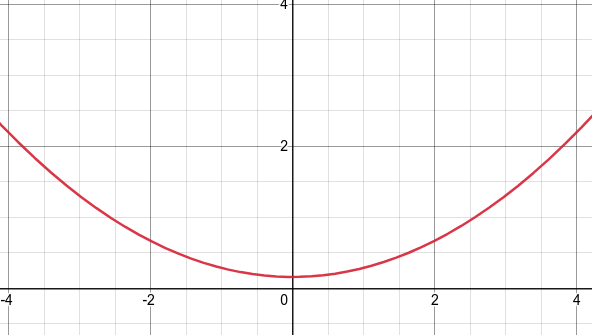
\includegraphics[width=\linewidth, height=5cm]{second.png} \caption{$\hat{f_{2}}$} \par
		\end{multicols}
	\end{figure}
	
	\noindent In the upper half of the plane, $\hat{f_{1}}$ looks approximately like a Gaussian distribution which the Maxwellian is for a distribution of velocity (not speed) for a fixed temperature. $\hat{f_{2}}$ is sort of the opposite of $\hat{f_{1}}$. But given that the functions are defined in a limited range, the integrals do not diverge.
	
	\subsubsection{A justification for Parabolic density functions - Vlasov equation}
	One good exercise is to check what happens when plugging in  $\hat{f_{1}}$ , $\hat{f_{2}}$ and $f_{M}$ in  the collisionless Vlasov equation. As discussed earlier Kinetic theory of plasma describes the system with a density function. The dynamics of the plasma is described by the changing of the density function. Earlier, Boltzmann equation was discussed as an equation used to describe this dynamics. Vlasov equation is an instance of the collisionless Boltzmann equation discussed earlier; where it is assumed that the particles do not interact with each other, and the force exerted on the particles is described by the Lorentz force. The Vlasov equation is written as:
	$$ \frac{\partial f}{\partial t} + \boldsymbol{v} \cdot \nabla f + \frac{q}{m} \left(\mathrm{\mathbf{E}}+\boldsymbol{v} \times \mathrm{\mathbf{B}} \right) \cdot {\partial}_{\boldsymbol{v}} f = 0 $$
	For all three of the density functions
	$$\frac{\displaystyle \partial f}{\displaystyle \partial t} = 0 \mathrm{,} \hspace{1cm} \frac{\displaystyle \partial f}{\displaystyle \partial x} = 0 \mathrm{,} \hspace{1cm} \frac{\displaystyle \partial f}{\displaystyle \partial y} = 0 \mathrm{,} \hspace{1cm} \frac{\displaystyle \partial f}{\displaystyle \partial z} = 0 $$ as all three have no explicit dependence on position or time. The Vlasov equation then becomes $$ \left(\mathrm{\mathbf{E}}+\boldsymbol{v} \times \mathrm{\mathbf{B}} \right) \cdot {\partial}_{\boldsymbol{v}} f = 0 $$ which is 
	$$ \left(E_{x} + v_{y} B_{z} - v_{z} B_{y}\right) \frac{\displaystyle \partial f}{\displaystyle \partial v_{x}} + \left(E_{y} + v_{z} B_{x} - v_{x} B_{z}\right) \frac{\displaystyle \partial f}{\displaystyle \partial v_{y}} + \left(E_{z} + v_{x} B_{y} - v_{y} B_{x}\right) \frac{\displaystyle \partial f}{\displaystyle \partial v_{z}} = 0$$
	For the Maxwellian, $$ 	\widehat{f_{M}} := \hat{f}(\boldsymbol{x}, \boldsymbol{v}, t) = \left(\frac{m}{2\pi KT}\right)^{\frac{3}{2}} \mathrm{exp}\left(-\frac{v^{2}}{v_{th}^{2}}\right) $$
	$$\frac{\displaystyle \partial f_{M}}{\displaystyle \partial v_{x}} = \left(\frac{m}{2 \pi K T}\right)^{\frac{3}{2}}  \mathrm{exp} \left(\frac{-v^{2}}{v_{th}^{2}}\right)\left(\frac{-2 v_{x}}{v_{th}^{2}}\right)\mathrm{,} \hspace{1cm} \frac{\displaystyle \partial f_{M}}{\displaystyle \partial v_{y}} = \left(\frac{m}{2 \pi K T}\right)^{\frac{3}{2}}  \mathrm{exp} \left(\frac{-v^{2}}{v_{th}^{2}}\right)\left(\frac{-2 v_{y}}{v_{th}^{2}}\right) \mathrm{,}$$ $$\frac{\displaystyle \partial f_{M}}{\displaystyle \partial v_{z}} = \left(\frac{m}{2 \pi K T}\right)^{\frac{3}{2}}  \mathrm{exp} \left(\frac{-v^{2}}{v_{th}^{2}}\right)\left(\frac{-2 v_{z}}{v_{th}^{2}}\right)$$
	plugging in, the equation becomes
	$$\left(\frac{m}{2 \pi K T}\right)^{\frac{3}{2}}  \mathrm{exp} \left(\frac{-v^{2}}{v_{th}^{2}}\right)\left(\frac{-2}{v_{th}^{2}}\right) \left[v_{x}\left( E_{x} + v_{y} B_{z} - v_{z} B_{y} \right) + v_{y} \left( E_{y} + v_{z} B_{x} - v_{x} B_{z} \right) + \right.$$ $$\left. v_{z} \left(E_{z} + v_{x} B_{y} - v_{y} B_{x}\right) \right] = 0$$
	which gives
	$$v_{x} E_{x} + v_{y} E{y} + v_{z} E_{z} = 0$$
	which can also be written as 
	$$
		\label{eqn:MaxwellInVlasov}
		\boldsymbol{v} \cdot \mathrm{\mathbf{E}} = 0
	$$ 
	which says that the particles move perpendicular to the electric field which is characteristic of the Lorentz force.
	For the parabolic functions,
	\[ \hat{f_{1}} = 
	\begin{cases} 
		\frac{1}{4 v_{a}^{3}} \left(1 - \frac{v^{2}}{2 v_{a}^2}\right) & -v_{a}\leq v\leq v_{a} \\
		0 & else 
	\end{cases}
	\]
	\[ \hat{f_{2}} = 
	\begin{cases}
		\frac{1}{12 v_{a}^{3}} \left(1 + \frac{v^{2}}{2 v_{a}^2}\right) & v_{a}\leq v\leq v_{a} \\
		0 & else
	\end{cases}\] 
	\[ \frac{\displaystyle \partial \hat{f_{1}}}{\displaystyle \partial v_{x}} = 
	\begin{cases} 
		\frac{1}{4 v_{a}^{3}} \left(\frac{- 2 v_{x}}{2 v_{a}^2}\right) & -v_{a} < v < v_{a} \\
		\mathrm{undefined} & v = - v_{a}, v = v_{a} \\
		0 & else 
	\end{cases}
	\]
	\[ \frac{\displaystyle \partial \hat{f_{1}}}{\displaystyle \partial v_{y}} = 
	\begin{cases} 
		\frac{1}{4 v_{a}^{3}} \left(\frac{- 2 v_{y}}{2 v_{a}^2}\right) & -v_{a} < v < v_{a} \\
		\mathrm{undefined} & v = - v_{a}, v = v_{a} \\
		0 & else 
	\end{cases}
	\]
	\[ \frac{\displaystyle \partial \hat{f_{1}}}{\displaystyle \partial v_{z}} = 
	\begin{cases} 
		\frac{1}{4 v_{a}^{3}} \left(\frac{- 2 v_{z}}{2 v_{a}^2}\right) & -v_{a} < v < v_{a} \\
		\mathrm{undefined} & v = - v_{a}, v = v_{a} \\
		0 & else 
	\end{cases}
	\]
	\[ \frac{\displaystyle \partial \hat{f_{2}}}{\displaystyle \partial v_{x}} = 
	\begin{cases} 
		\frac{1}{12 v_{a}^{3}} \left(\frac{2 v_{x}}{2 v_{a}^2}\right) & -v_{a} < v < v_{a} \\
		\mathrm{undefined} & v = - v_{a}, v = v_{a} \\
		0 & else 
	\end{cases}
	\]
	\[ \frac{\displaystyle \partial \hat{f_{2}}}{\displaystyle \partial v_{y}} = 
	\begin{cases} 
		\frac{1}{12 v_{a}^{3}} \left(\frac{2 v_{y}}{2 v_{a}^2}\right) & -v_{a} < v < v_{a} \\
		\mathrm{undefined} & v = - v_{a}, v = v_{a} \\
		0 & else 
	\end{cases}
	\]
	\[ \frac{\displaystyle \partial \hat{f_{2}}}{\displaystyle \partial v_{z}} = 
	\begin{cases} 
		\frac{1}{12 v_{a}^{3}} \left(\frac{2 v_{z}}{2 v_{a}^2}\right) & -v_{a} < v < v_{a} \\
		\mathrm{undefined} & v = - v_{a}, v = v_{a} \\
		0 & else 
	\end{cases}
	\]
	In the range $v \in \mathbb{R} \textbackslash \left[-v_{a}, v_{a}\right] $ the equation becomes $0 = 0$ which is trivial. The equation becomes undefined for $v = v_{a}$ and 
	$v = - v_{a}$ but we can ignore that for now. In the interesting range of $v \in \left(-v_{a}, v_{a}\right) $, the equation becomes 
	$$ \frac{1}{4 v_{a}^{3}} \left(\frac{- 2}{2 v_{a}^2}\right) \left[v_{x}\left( E_{x} + v_{y} B_{z} - v_{z} B_{y} \right) + v_{y} \left( E_{y} + v_{z} B_{x} - v_{x} B_{z} \right) + v_{z} \left(E_{z} + v_{x} B_{y} - v_{y} B_{x}\right) \right] = 0 $$
	for $\hat{f_{1}}$ and
	$$ \frac{1}{12 v_{a}^{3}} \left(\frac{2}{2 v_{a}^2}\right) \left[v_{x}\left( E_{x} + v_{y} B_{z} - v_{z} B_{y} \right) + v_{y} \left( E_{y} + v_{z} B_{x} - v_{x} B_{z} \right) + v_{z} \left(E_{z} + v_{x} B_{y} - v_{y} B_{x}\right) \right] = 0 $$
	for $\hat{f_{2}}$ which both give the same equation as $\widehat{f_{M}}$
	$$v_{x} E_{x} + v_{y} E{y} + v_{z} E_{z} = 0 \hspace{1cm}\mathnormal{or}\hspace{1cm}\boldsymbol{v} \cdot \mathrm{\mathbf{E}} = 0$$
	\noindent $\hat{f_{1}}$ and $\hat{f_{2}}$ behave similar to $\hat{f_{M}}$ when plugged into the Vlasov equation.
	
	\subsubsection{A justification for Parabolic density functions - Magnetic mirror}
	\noindent Since the quantity $\frac{\displaystyle sin^{2}\theta}{\displaystyle B_{z}}$ is conserved in a magnetic mirror, it is a good exercise to calculate the average value or expectation of $sin^{2}\theta$, $\left\langle sin^{2}\theta\right\rangle = \left\langle \frac{\displaystyle v_{\perp}^{2}}{\displaystyle v^{2}}\right\rangle = \left\langle \frac{\displaystyle v_{x}^{2} + v_{y}^{2}}{\displaystyle v_{x}^{2} + v_{y}^{2} +  v_{z}^{2}}\right\rangle $ 
	For the Maxwellian $\widehat{f_{M}}$,
	$$\left\langle \frac{\displaystyle v_{x}^{2} + v_{y}^{2}}{\displaystyle v_{x}^{2} + v_{y}^{2} +  v_{z}^{2}}\right\rangle = \left(\frac{m}{2\pi KT}\right)^{\frac{3}{2}} $$ 
	$$ \int_{v_{x} = - \infty}^{v_{x} = \infty} d v_{x} \int_{v_{y} = - \infty}^{v_{y} = \infty} d v_{y} \int_{v_{z} = - \infty}^{v_{z} = \infty} d v_{z} \left( \frac{\displaystyle v_{x}^{2} + v_{y}^{2}}{\displaystyle v_{x}^{2} + v_{y}^{2} + v_{z}^{2}} \right)  \mathrm{exp}\left(-\frac{v_{x}^{2}}{v_{th}^{2}}\right) \mathrm{exp}\left(-\frac{v_{y}^{2}}{v_{th}^{2}}\right) \mathrm{exp}\left(-\frac{v_{z}^{2}}{v_{th}^{2}}\right)$$
	Likewise for the parabolic functions,
	$$\left\langle \frac{\displaystyle v_{x}^{2} + v_{y}^{2}}{\displaystyle v_{x}^{2} + v_{y}^{2} +  v_{z}^{2}}\right\rangle = \frac{1}{4 v_{a}^{3}} $$ $$\int_{v_{x} = - v_{a}}^{v_{x} = v_{a}} d v_{x} \int_{v_{y} = - v_{a}}^{v_{y} = v_{a}} d v_{y} \int_{v_{z} = - v_{a}}^{v_{z} = v_{a}} d v_{z} \left( \frac{\displaystyle v_{x}^{2} + v_{y}^{2}}{\displaystyle v_{x}^{2} + v_{y}^{2} + v_{z}^{2}} \right)  \left(1 - \frac{v_{x}^{2}}{2 v_{a}^2} - \frac{v_{y}^{2}}{2 v_{a}^2} - \frac{v_{z}^{2}}{2 v_{a}^2} \right) $$
	for $\hat{f_{1}}$ and
	$$\left\langle \frac{\displaystyle v_{x}^{2} + v_{y}^{2}}{\displaystyle v_{x}^{2} + v_{y}^{2} +  v_{z}^{2}}\right\rangle = \frac{1}{12 v_{a}^{3}} $$ $$\int_{v_{x} = - v_{a}}^{v_{x} = v_{a}} d v_{x} \int_{v_{y} = - v_{a}}^{v_{y} = v_{a}} d v_{y} \int_{v_{z} = - v_{a}}^{v_{z} = v_{a}} d v_{z} \left( \frac{\displaystyle v_{x}^{2} + v_{y}^{2}}{\displaystyle v_{x}^{2} + v_{y}^{2} + v_{z}^{2}} \right)  \left(1 + \frac{v_{x}^{2}}{2 v_{a}^2} + \frac{v_{y}^{2}}{2 v_{a}^2} + \frac{v_{z}^{2}}{2 v_{a}^2} \right) $$
	for $\hat{f_{2}}$ which are all very difficult to evaluate because of the denominators. \\
	\noindent So an approximation $\left\langle \frac{\displaystyle v_{x}^{2} + v_{y}^{2}}{\displaystyle v_{x}^{2} + v_{y}^{2} +  v_{z}^{2}}\right\rangle =  \frac{\displaystyle \left\langle v_{x}^{2} + v_{y}^{2}\right\rangle}  {\displaystyle \left\langle v_{x}^{2} + v_{y}^{2} +  v_{z}^{2}\right\rangle} + c_{0}$ can be done where $c_{0}$ is an error term.\\
	
	\noindent For $\widehat{f_{M}}$, $\displaystyle \left\langle v_{x}^{2} + v_{y}^{2}\right\rangle = \frac{\displaystyle 2 K T}{\displaystyle m}$ and $\left\langle v_{x}^{2} + v_{y}^{2} +  v_{z}^{2}\right\rangle = \frac{\displaystyle 3 K T}{\displaystyle m}$ so $$\left\langle sin^{2}\theta\right\rangle = \left\langle \frac{\displaystyle v_{\perp}^{2}}{\displaystyle v^{2}}\right\rangle = \left\langle \frac{\displaystyle v_{x}^{2} + v_{y}^{2}}{\displaystyle v_{x}^{2} + v_{y}^{2} +  v_{z}^{2}}\right\rangle = \frac{\displaystyle \left\langle v_{x}^{2} + v_{y}^{2}\right\rangle}  {\displaystyle \left\langle v_{x}^{2} + v_{y}^{2} +  v_{z}^{2}\right\rangle} + c_{0} = \frac{2}{3} + c_{0}$$
	For $\hat{f_{1}}$, $\displaystyle \left\langle v_{x}^{2} + v_{y}^{2}\right\rangle = \frac{22}{45} v_{a}^2$ and $\displaystyle \left\langle v_{x}^{2} + v_{y}^{2} +  v_{z}^{2}\right\rangle = \frac{11}{15} v_{a}^2$ so $\displaystyle \left\langle sin^{2}\theta\right\rangle = \frac{2}{3} + c_{0}$ and \vspace{0.2cm} \\
	\noindent For $\hat{f_{2}}$, $\displaystyle \left\langle v_{x}^{2} + v_{y}^{2}\right\rangle = \frac{98}{135} v_{a}^2$ and $\displaystyle \left\langle v_{x}^{2} + v_{y}^{2} +  v_{z}^{2}\right\rangle = \frac{49}{45} v_{a}^2$ so $\displaystyle \left\langle sin^{2}\theta\right\rangle = \frac{2}{3} + c_{0}$ \\
	\noindent $\hat{f_{1}}$ and $\hat{f_{2}}$ behave similar to $\widehat{f_{M}}$ when plugged into the expression for $\left\langle sin^{2}\theta\right\rangle$. \\
	
	\noindent Since $\hat{f_{1}}$ and $\hat{f_{2}}$ behave similar to $\widehat{f_{M}}$ when plugged into the Vlasov equation and the expression for $\left\langle sin^{2}\theta\right\rangle$, it seems that $\hat{f_{1}}$ and $\hat{f_{2}}$ are nice distribution functions to work with.
	
	
	\subsection{Fields}
	In order to define the plasma chamber and hence the control on the plasma, we are interested in defining a few different electric and magnetic field configurations. We have a few different field configurations in mind. For the electric field, as of now we have 2 field configurations:
	\begin{enumerate}
		\item \textbf{Uniform electric field} \\
		The electric field has the same value everywhere. It is a very simple configuration to think about and use.
		\item \textbf{Electric field due to an electrode} \\
		We describe the electrode in the following way: Every particle sees the electrode create an electric field created by a pair of capacitor plate at a distance taken only in the $x$-$y$ plane. This is to say that every point on the electrode; now assumed to be a line along the $z$-direction, creates an electric field like that created between a pair of capacitor plates, if there is a particle at the same $z$-coordinate as that point. So currently we use the expression $\mathbf{E} = V \cdot d\boldsymbol{r}$ where $d\boldsymbol{r}$ is a vector whose $z$-coordinate is zero.
		
	\end{enumerate}
	For the magnetic field, we have 3 configurations as of now:
	\begin{enumerate}
		\item \textbf{Uniform magnetic field} \\
		The uniform magnetic field has the same value everywhere. It is very simple to understand and use.
		\item \textbf{Magnetic field due to a Helmholtz coil} \\
		The magnetic field strength due to a Helmholtz coil is given by the expression:
		$$B = \left(\frac{4}{5}\right)^{3/2} \frac{\mu_{0} n I}{R}$$
		We may use the axis of the coil as the direction of the field.
		\item \textbf{Magnetic field due to 2 Helmholtz coils} \\
		The magnetic field due to two Helmholtz coils is calculated by simply adding the magnetic fields created by the two coils.
	\end{enumerate}
	
	\subsection{Running different batches}
	As discussed earlier we would like to describe different batches of particles, so as to model plasma streams; where the particles are sent into the chamber based on different initialization strategies. The particles are then evolved based on the Boris algorithm. We would then remove the particles to simulate particles exiting the chamber, or being absorbed to form coatings as in different surface engineering processes like Magnetron Sputtering.
	
	\section{Work carried out so far}
	The simulation is programmed in jupyter notebook files (.ipynb extensions) that run python and markdown. The notebooks are available in the following Github repository, in the notebooks folder.
	
	\begin{center}
		\begin{tcolorbox}[width=15cm]
			GitHub repository:
			\vspace{0.2cm} 
			\phantom{a} \\
			\phantom{push this repository}
			\textbf{\textit{https://github.com/18BME2104/MagneticMirror}} \\
			\phantom{a}
		\end{tcolorbox}
	\end{center}
	
	\textbf{Algorithm Outline} \\
	Different aspects of the program are discussed based on the different notebooks (ipynb files) that describe them.
	\begin{center}
		\begin{tcolorbox}[width=12cm]
			Required functionalities and Files:
			\vspace{0.2cm} 
			\begin{enumerate}
				\item Constants - \textbf{constants.ipynb}
				\item Particle - \textbf{particle.ipynb}
				\item Electric and Magnetic fields - \textbf{field.ipynb}
				\item Particle initialization - \textbf{sampling.ipynb}
				\item Updating the particles - \textbf{step.ipynb}
				\item Batches of updates - \textbf{run.ipynb}
				\item Plotting - \textbf{plot.ipynb}
			\end{enumerate}
		\end{tcolorbox}
	\end{center}
	
	\subsection{Constants - constants.ipynb}
	The \textbf{constants.ipynb} notebook describes some constants useful in the program. Some useful constants are $e$ (electron charge) $m_{e}$ (electron mass), charges and masses of ions in the plasma, $a.m.u$ (atomic mass unit), $N_{A}$ (Avogadro's number), $\epsilon_{0}$ (permittivity of vacuum), $\mu_{0}$ (permeability of vacuum), $K$ or $k_{B}$ (Boltzmann's constant), etc.
	
	\lstinputlisting[language=Python, linerange={1-6}]{constants.py}
	
	\subsection{Particle - particle.ipynb}
	The \textbf{particle.ipynb} notebook describes the state of a particle; its position, velocity, mass, charge, name, and optionally acceleration (which is set to 0 as default if it is not required to track the acceleration of a particle) as of now. \\
	
	\noindent Currently the \textbf{Boris algorithm} as discussed earlier, is an update strategy defined to update the state of a particle. Other strategies could be defined in new functions in the class. However, Boris algorithm is good enough for us to get started.
	
	\lstinputlisting[language=Python]{particle.py}
	
	\subsection{Electric and Magnetic fields - field.ipynb}
	Electric and Magnetic field configurations described in \textbf{field.ipynb}. \\
	
	\noindent Currently \textbf{Uniform Electric field} and the \textbf{Radial Electric field} (the field depends on the particle's position) created by an electrode are available to set up electric fields. \textbf{Uniform Magnetic field} and Magnetic field created by a \textbf{Helmholtz coil} and that by two Helmholtz coils are available. \\
	
	\noindent Other Electric and Magnetic fields can be defined as functions in this class. These fields could be based on modeling of apparatus used to create electric or magnetic fields such as coils, or based on analytic expressions.
	
	
	\lstinputlisting[language=Python]{field.py}
	
	
	\subsection{Particle initialization - sampling.ipynb}
	The initial positions and velocities of the particles play an important role in the evolution of their state under the influence of electric and magnetic fields. The initial distribution of positions and velocities define where the particles start in the setup (or lab apparatus); for example where they are injected into a sputtering chamber through valves, and what velocities they start with; for example what potential they are accelerated through or what parameters were used for the pumps used to pump the particles in.\\
	
	\noindent The tracking of initial distribution is also important in determining how the magnetic mirror effect is observed in the plasma. The Sampler class samples initial positions and velocities for a given number of particles based on some available schemes. \\
	
	\noindent Currently positions can be sampled such that all particles start at the \textbf{same position} (like for example if injected through a port), \textbf{at the same distance} but randomly distributed in angular positions relative to some point(origin as of now). Velocities can be sampled such that particles have the \textbf{same speed}, \textbf{same velocity} or \textbf{Maxwellian distributed speeds} or \textbf{Maxwellian distributed velocities}.   
	
	\lstinputlisting[language=Python, linerange={1-68, 77-77}]{sampling.py}
	% assert keyword causes some error 
	% WARNING:
	% changing code in sampling.py requires chaging
	% line numbers here 
	
	\noindent The initial positions and velocities could be passed around in lists but to be able to reuse some generated samples, and avoid sampling all the time, it is convenient to write sampled positions and velocities to files (csv format seems convenient). This functionality is described as:
	\lstinputlisting[language=Python, linerange={1-3, 69-77}]{sampling.py}
	% assert keyword causes some error 
	% WARNING:
	% changing code in sampling.py requires chaging
	% line numbers here 
	
	\subsection{Updating the particles - step.ipynb}
	The Step class is concerned with \textbf{initializing particles}, \textbf{defining the fields}, and \textbf{updating the states of the particles} (positions and velocities) under the action of electric and magnetic fields.
	\lstinputlisting[language=Python, linerange={1-20, 27-27}]{step.py}
	
	\noindent To use sampled positions and velocities that have been saved in csv files, some reading functionality is useful to load these positions and velocities to be used during initialization.
	\lstinputlisting[language=Python, linerange={1-3, 21-27}]{step.py}
	
	\section{Work to be done}
	Work on the \textbf{constants.ipynb}, \textbf{particle.ipynb}, \textbf{fields.ipynb} and \textbf{sampling.ipynb} has been done to a certain extent. Basic work on \text{step.ipynb} has been done. However, we could modify functionalities defined here and add other definitions as work on \textbf{run.ipynb} progresses, so that everything works well together. \\
	Other functionalities that could be added are:
	\begin{enumerate}
		\item \textbf{Sampling} \\
		Sampling strategies based on parabolic density functions discussed earlier are yet to be defined. New sampling strategies such as one initializing particles with the same Kinetic energy; as would happen if particles (of possibly different species) were accelerated through the same potential difference, could be defined.
		\item \textbf{Fields} \\
		New field configurations could be defined. We could also modify existing field configuration like the Electric field due to an electrode; if we find a different expression to describe it better, or if the current expression does not work well.
	\end{enumerate}
	However, we do not yet have a plasma simulation running. The major portion of the work to be done to achieve this includes working on the \textbf{run.ipynb} notebook. To be able to understand the simulation; to check if works correctly and to understand the plasma behavior, we also need to define functionalities to plot different parameters like particle positions and velocities. These functionalities will be defined in \textbf{plot.ipynb} notebook, which can be imported into \textbf{ryn.ipynb} and \textbf{step.ipynb} notebooks to plot these quantities when the simulation is running, or from saved data. 
	
	\subsection{Batches of updates - run.ipynb}
	The Run class is concerned with running the steps defined by the Step class in step.ipynb. This includes creating batches of particles, updating them under the influence of electric and magnetic fields and removing them if they move out of the region of interest or for example are absorbed during a coating process. New batches of particles can be created to model the flow of particles as in a plasma chamber setup. Functionality to change the fields; for example changing the Voltages in electrodes or Currents in the coils, are also defined. This better models the control of plasma supply and electric and magnetic field control apparatus as in a laboratory.
	\lstinputlisting[language=Python]{run.py}
	
	\subsection{Plotting - plot.ipynb}
	The plot class is used to define functionalities to draw particle positions, plot positions and velocities of particles, as the system evolves like a lab apparatus. These functionalities are imported into run.ipynb; and if required other notebooks, to be used when the simulation is running; or optionally from saved data. Work on this notebook is yet to be started.
	
	\subsection{Understanding of the plasma}
	The big question, is that once we have a simulation running, how do we do analysis on the plasma so that the project helps improve our understanding of a plasma system? The sampling aspect of the project, will allow us to understand how different parameters of the plasma like the temperature; when it enters the chamber affect the behavior of the plasma. We can also study for example, the velocity distribution of the particles as they evolve in the chamber. Studying different field configurations; even simple functionalities like being able to change the Voltage of an electrode to change the electric field- like one might with a real apparatus, will help us understand the behavior of plasma under different or changing fields. \\
	\noindent Such strategies will allow us to understand how to contain a plasma in chamber; and one such instance would be a magnetron sputtering chamber where one could study the magnetic mirror effect. The magnetic mirror effect in a magnetron sputtering chamber serves as one example of studies we could do on the plasma parameters, studying a plasma in simulation. So our title serves as an example for what we could do with such a project. We have learned through the course of doing the project that more could be achieved with such a system than what we initially planned to focus on. 
	
	\section{Gantt Chart (Work Plan)}
	\begin{figure}
		\begin{ganttchart}[vgrid, hgrid]{1}{18}
			\gantttitle{January}{5} 
			\gantttitle{February}{4}
			\gantttitle{March}{4}
			\gantttitle{April}{4}
			\gantttitle{May}{1}\\
			\gantttitlelist{1,...,18}{1}\\
			%First Group
			\ganttgroup{Review 1}{1}{6} \\
			\ganttbar{$\mathnormal{Study:\; plasma\; models,\; kinetic\; theory}$}{1}{2} \\
			\ganttbar{$\mathnormal{Study:\; PIC,\; Boris\; Algorithm}$}{2}{3} \\
			\ganttbar{$\mathnormal{Algorithm:\; idea,\; constants}$}{3}{4}\\
			\ganttmilestone{$\mathbf{Milestone\; 1:\; Algorithm\; start}$}{3}\\
			\ganttbar{$\mathnormal{Algorithm:\; particle,\; field,\; step}$}{4}{5}\\
			\ganttbar{$\mathnormal{Algorithm:\; sampling,\; Review\; preparation}$}{5}{6}\\
			%\ganttlink{elem0}{elem1}
			%\ganttmilestone{Milestone 1}{11}\\
			%Second Group
			\ganttgroup{Review 2}{7}{12} \\
			\ganttbar{$\mathnormal{Algorithm:\; run,\; plot}$}{7}{8} \\
			\ganttbar{$\mathnormal{Algorithm:\; changes\; and\; fixes}$}{8}{9}\\
			\ganttbar{$\mathnormal{First\; plasma\; simulation}$}{9}{10}\\
			\ganttmilestone{$\mathbf{Milestone\; 2:\; Simulation\; running}$}{9}\\
			\ganttbar{$\mathnormal{First\; results\; and\; study}$}{10}{11}\\
			\ganttbar{$\mathnormal{Review\; preparation}$}{11}{12}\\
			%\ganttlink{elem4}{elem5}
			%\ganttmilestone{Milestone 1}{11}
			%Third Group
			\ganttgroup{Review 3}{13}{18} \\
			\ganttbar{$\mathnormal{Definitions:\; fields,\; density\; functions}$}{13}{14} \\
			\ganttbar{$\mathnormal{Fixes\; and\; study}$}{14}{15} \\
			\ganttmilestone{$\mathbf{Milestone\; 3:\; Study\; and\; understanding}$}{15}\\
			\ganttbar{$\mathnormal{Study\; and\; result\; analysis}$}{15}{16} \\
			\ganttbar{$\mathnormal{Report\; and\; review\; preparation}$}{16}{18}
			%\ganttlink{elem8}{elem9}
			%\ganttmilestone{Milestone 1}{11}
		\end{ganttchart}
	\caption{Gantt chart}
	\end{figure}
	\clearpage
	
	\textbf{Progress description:}
	\begin{itemize}
		\item \textbf{Review 1}
	\end{itemize}
	\begin{enumerate}
		\item Weeks 1-2 \textbf{Study: plasma models, kinetic theory} \\
		We first studied basic plasma physics, and a bit more on the kinetic theory of plasma as that seemed relevant to our project.
		\item Weeks 2-3 \textbf{Study: PIC, Boris Algorithm} \\
		We then studied particle in cell methods and then the Boris Algorithm. 
		\item Weeks 3-4 \textbf{Algorithm: idea, constants}\\
		With some idea of how to proceed with the project, we started working on the algorithm. We started by with work on the \textbf{constants.ipynb} notebook, defining the constants that might be needed for the project.
		\item Weeks 4-5 \textbf{Algorithm: particle, field, step}\\
		We then worked on the notebook \textbf{particle.ipynb} where we defined a particle and how to update it. In the \textbf{field.ipynb} file, we worked to define some basic field configurations. Then we worked on \textbf{step.ipynb} to define steps of evolutions of the particles in a field configuration. This is the basic work on single particle dynamics.
		\item Weeks 5-6 \textbf{Algorithm: sampling, Review preparation}\\
		We then worked on some kinetic theory aspects of the project, defining some sampling strategies based on the Uniform velocity and Maxwellian distribution. We then started preparing for review 1.
	\end{enumerate}
	\begin{itemize}
		\item \textbf{Review 2}
	\end{itemize}
		\begin{enumerate}
			\item Weeks 7-8 \textbf{Algorithm: run, plot} \\
			We plan to work next on \textbf{run.ipynb} to define running of batches of particle evolution and on \textbf{plot.ipynb} to define plot functionalities.
			\item Weeks 8-9 \textbf{Algorithm: changes and fixes}\\
			We anticipate that there may be errors in the programs that we will need some time to debug.
			\item Weeks 9-10 \textbf{First plasma simulation}\\
			We then expect to have the first plasma simulation running.
			\item Weeks 10-11 \textbf{First results and study}\\
			Running some plasma simulations, we intend to study the first set of results.
			\item Weeks 11-12 \textbf{Review preparation}\\
			We plan to prepare for review 2 based on some preliminary results and understanding.
		\end{enumerate}
		\begin{itemize}
			\item \textbf{Review 3}
		\end{itemize}
		\begin{enumerate}
			\item Weeks 13-14 \textbf{Definitions: fields, density functions}\\
			We then intend to make some new definitions like sampling based on the parabolic density functions, some new field configurations and possibly some new functionality handling particle states.
		\item Weeks 14-15 \textbf{Fixes and study}\\
		We expect to spend some time making final fixes and changes on the algorithm. We then turn to studying the results.
		\item Weeks 15-16 \textbf{Study and result analysis}\\
		We intend to spend some time studying the results and trying to understand the plasma model in the simulation.
		\item Weeks 16-18 \textbf{Report and review preparation}\\
		We then expect to start preparing for review 3, and preparation of the report and other documents.
		\end{enumerate}
	
	\section{Milestones in the project phase}
	\begin{enumerate}
		\item[Milestone 1] \textbf{Algroithm start} \hspace*{\fill} Week 3 - \textbf{Achieved}\\
		Around week 3 we had some understanding of basic plasma physics and so started working on how to formulate the problem as an algorithm. \hspace*{\fill} Before review 1
		\item[Milestone 2] \textbf{Simulation runnning}
		\hspace*{\fill} Week 9 - \textbf{Expected}\\
		We expect to have the simulation running around week 9 of the project. This will allow us to have some preliminary results and understanding of our model, by review 2. \hspace*{\fill} Before review 2 \phantom{a}
		\item[Milestone 3] \textbf{Study and understanding}	
		\hspace*{\fill} Week 15 - \textbf{Expected} \\
		We intend to perform study on plasma using our algorithm and improve our understanding of a plasma and how to control and study a plasma system before the end of the project. \hspace*{\fill} Before review 3
	\end{enumerate}
	
	
	\begin{thebibliography}{}
		\bibitem{SurfaceEng}
		Professor Sitaram Dash. (Fall Semester 2021). \textit{MEE4005 Surface Engineering} (lecture notes). SMEC, VIT Vellore.
		\bibitem{MKunz}
		Matthew W. Kunz. (November 9, 2020). \textit{Introduction to Plasma Astrophysics} (lecture notes). Princeton Plasma Physics Laboratory.
		\bibitem{chenbook}
		Chen, F. F. (1984). \textit{Introduction to plasma physics and controlled fusion} (Vol. 1, pp. 8-11). New York: Plenum press.
		\bibitem{mirror1}
		Na, Yong-Su (2017). \textit{Introduction to nuclear fusion} (Lecture 9 Mirror, lecture slide). Seoul National University Open Courseware.
		\bibitem{mirror2}
		F\"{o}rel\"{a}sning (2009). \textit{Charged particle motion in magnetic field} (lecture slide). Lule\"{a} University of Technology.
		\bibitem{PIC good}
		Myers, A., Colella, P., \& Straalen, B. V. (2017). \textit{A 4th-Order Particle-in-Cell Method with Phase-Space Remapping for the Vlasov--Poisson Equation}. SIAM Journal on Scientific Computing, 39(3), B467-B485.
		\bibitem{PIC IAS}
		Anatoly Spitkovsky (2016). \textit{Kinetic plasma simulations} (lecture slide). PiTP 2016 on Computational Plasma Astrophysics. Institute for Advanced Study.
		\bibitem{Borisgood}
		Qin, H., Zhang, S., Xiao, J., $\&$ Tang, W. M. (April, 2013). \textit{Why is Boris algorithm so good?}. Princeton Plasma Physics Laboratory, PPPL-4872.
		
	\end{thebibliography}

\end{document}